%% -*- coding:utf-8 -*-
\chapter{练习题答案}
%\chapter{Solutions to the exercises}

\section{导言与术语}
%\section{Introduction and basic terms}

\eal
\ex \field{Karl}{VF} \field{isst}{LS}.
\ex \field{Der Mann}{VF} \field{liebt}{LS} \field{eine Frau}{MF}, \field{\field{den}{VF} \field{Peter}{MF} \field{kennt}{RS}}{NF}.
\ex \field{Der Mann}{VF} \field{liebt}{LS} \field{eine Frau, \field{die}{VF} \field{Peter}{MF} \field{kennt}{RS}}{MF}.
%\ex \field{Die Studenten}{VF} \field{behaupten}{LS}, \field{\field{nur wegen der Hitze}{MF} \field{einzuschlafen}{RS}}{MF}.
\ex \field{Die Studenten}{VF} \field{haben}{LS} \field{behauptet}{RS}, \field{\field{nur wegen der Hitze}{MF} \field{einzuschlafen}{RS}}{NF}.
\ex \field{\field{Dass}{LS} \field{Peter nicht}{MF} \field{kommt}{RS}}{VF}, \field{ärgert}{LS} \field{Klaus}{MF}.
\ex \field{\field{Einen Mann}{MF} \field{küssen}{RS}, \field{\field{der}{VF} \field{ihr nicht}{MF} \field{gefällt}{RS}}{NF}}{VF}, \field{würde}{LS} \field{sie nie}{MF}.
\zl
对于(\mex{0}c)而言:理论上,这也可以是关系小句外置到后场的一个例子。因为eine Frau, die Peter kennt (Peter认识的一个女人)是一个组成成分,不过,一般认为这个关系小句并没有重新排序。相反,我们有一个更简单的结构,它把eine Frau, die Peter kennt作为一个完整的NP放在中场的位置上。
%On (\mex{0}c): theoretically, this could also be a case of extraposition of the relative clause to
%the postfield. Since \emph{eine Frau, die Peter kennt} is a constituent, however, it is assumed that
%no reordering of the relative clause has taken place. Instead, we have a simpler structure with
%\emph{eine Frau, die Peter kennt} as a complete NP in the middle field.


\section{短语结构语法}
%\section{Phrase structure grammars}

\begin{enumerate}
\item 任何一种文法都有可能提出额外的符号和规则,可能是会生成多余的结构,或者是根本没用过,因为规则的右手边没有能够使用的词或短语。比如说,如果我们在文法中加入下面的规则,我们需要一个仍能分析这个相同的语言片段的更为复杂的文法。
%\item For any grammar, it is possible to assume additional symbols and rules that create unnecessary structure or are simply
%never used because there are no words or phrases that could be used on the right"=hand side of the rule. If we were to add
%the following rule to our grammar, for example, we would have a more complex grammar that can still analyze the same fragment
%of the language.
\ea
Tralala $\to$ Trulla Trololo
\z
% \item Stellen Sie Überlegungen dazu an, wie man ermitteln kann, welche der unendlich vielen Grammatiken
%       die beste ist bzw.\ welche der Grammatiken die besten sind.
\item 一般认为,有着最少规则的文法是最好的。这样,我们可以拒用那些像(\mex{0})一样包括不必要规则的文法。
%\item In general, it is assumed that the grammar with the fewest rules is the best one. Therefore, we can reject grammars that
%contain unnecessary rules such as (\mex{0}).

\par\setlength\parindent{2em}
我们需要牢记,文法理论的目的是什么。如果我们的目标是为了描写人类的语言能力,那么有着更多规则的文法就比那些具有较少规则的文法要好。这是因为心理语言学的研究显示我们的大脑易储存高频的单位,而且并不是每次都由它们的个别部分构成,尽管我们当然有能力这么做。
%One should bear in mind what the aim of a theory of grammar is. If our goal is to describe the human
%language capacity, then a grammar with more rules could be better than other grammars with less
%rules. This is because psycholinguistic research has shown that highly"=frequent units are simply
%stored in our brains and not built up from their individual parts each time, although we would of
%course be able to do this.\todostefan{Quelle und Beispiel}

\item 这里的问题是有可能生成一个完整的空名词短语(见图\vref{Abbildung-leere-NP})。
%\item The problem here is the fact that it is possible to derive a completely empty noun phrase
% (see Figure~\vref{Abbildung-leere-NP}). 
\begin{figure}
\centering
\begin{forest}
sm edges
[NP
  [Det [\trace]]
  [\nbar
    [N [\trace]]]]
\end{forest}
\caption{\label{Abbildung-leere-NP}不带限定词和名词的名词短语}
%\caption{\label{Abbildung-leere-NP}Noun phrases without a visible determiner and noun}
\end{figure}%
这个名词短语可以被插进填充的NP所在的所有位置上。那么,我们可以分析例(\mex{1})这样的词的序列,其中schläft(睡觉)的主语被实现为一个空NP:
%This noun phrase could be inserted in all positions where an otherwise filled NP would have to stay. Then, we would
%be able to analyze sequences of words such as (\mex{1}), where the subject of \emph{schläft} `sleeps' is realized
%by an empty NP:
\ea[*]{
\gll Ich glaube, dass schläft.\\
     我 认为 \textsc{comp} 睡觉\\
%     I believe that sleeps\\
}
\z
\par\setlength\parindent{2em}
这个问题可以使用一个特征来解决,这个特征决定了\nbar 的左边界是否是空的。至少带一个形容词的可见的N和\nbar 具有“--” 值,其他的是“+”。空限定语就只能跟具有“--” 值的\nbar{}相组合。参见 \citew{Netter94}。
%This problem can be solved using a feature that determines whether the left periphery of the \nbar is empty.
%Visible Ns and \nbar with at least an adjective would have the value `--' and all others `+'. Empty determiners
%could then only be combined with \nbar{}s that have the value `--'. See  \citew{Netter94}.

\item 如果Bücher(书)在词库中是一个名词,那么为了使得诸如(\mex{1})的短语是可分析的,interessant(有趣的)这类形容词就需要修饰NPs。
%\item %Überlegen Sie, warum es nicht sinnvoll ist, \emph{Bücher} als NP ins Lexikon zu schreiben.
%If \emph{Bücher} `books' were an NP in the lexicon, then adjectives such as \emph{interessant} `interesting' would have to modify
%NPs in order for phrases such as (\mex{1}) to be analyzed.
\ea
\gll interessante Bücher\\
     有趣的 书\\
%     interesting books\\
\z
\par\setlength\parindent{2em}
不过,如果形容词跟名词短语组合,仍要解释例(\mex{1})为什么是不合乎语法的。
%If adjectives are combined with NPs, however, it still has to be explained why (\mex{1}) is ungrammatical.
\ea[*]{
\gll interessante die Bücher\\
     有趣的 \textsc{art}.\textsc{def} 书\\
%     interesting the books\\
}
\z
\par\setlength\parindent{2em}
有关这个话题的详细讨论,见 \citew[\S~6.6.2]{MuellerLehrbuch1}。\nocite{MuellerLehrbuch1}
%For a detailed discussions of this topic, see  \citew[Section~6.6.2]{MuellerLehrbuch1}.\nocite{MuellerLehrbuch1}

\item %% Überlegen Sie, warum es auch nicht sinnvoll ist, die folgende Regel für Nomina wie \emph{Bücher} anzunehmen:
%% \ea
%% NP $\to$ Modifikator* Bücher Modifkator*
%% \z

这类规则不能分析(\mex{1})中的那些名词短语:
%This kind of rule cannot analyze noun phrases such as those in (\mex{1}):
\eal
\ex 
\gll interessante [Aufsätze und Bücher]\\
     有趣的 \spacebr{}文章 和 书\\
%     interesting \spacebr{}essays and books\\
\ex 
\gll interessante [Aufsätze und Bücher aus Stuttgart]\\
     有趣的 \spacebr{}文章 和 书 来自 斯图加特\\
%     interesting \spacebr{}essays and books from Stuttgart\\
\zl
\par\setlength\parindent{2em}
由于形容词只能跟名词直接组合,这些短语就是无法分析的。Bücher(书)或Bücher aus Stuttgart(来自斯图加特的书)就是完整的名词短语了。因为一般认为并列成分要求具有相同的句法范畴,所以Aufsätze(文章)就应该是一个名词短语。Aufsätze und Bücher(文章和书)和Aufsätze und Bücher aus
  Stuttgart(来自斯图加特的文章和书)也应该是名词短语,这样还是没有解释为什么形容词跟这个名词组合。因为(\mex{-1})的关系,我们必须排除那些假定完整的名词短语跟形容词组合的分析。
%Since adjectives can only be combined directly with nouns, these phrases cannot be analyzed. 
 %\emph{Bücher} `books' or \emph{Bücher aus Stuttgart} `books from Stuttgart' would be complete NPs.
% Since it is assumed that coordinated elements always have the same syntactic category, then \emph{Aufsätze} `essays'
% would have to be an NP. \emph{Aufsätze und Bücher} and \emph{Aufsätze und Bücher aus
%  Stuttgart} would then also be NPs and it remains unexplained how an adjective can be combined with this NP.
%Because of (\mex{-1}), we must rule out analyses that assume that full NPs combine with adjectives.

\par\setlength\parindent{2em}
关于空成分的概括性论述见第\ref{chap-empty}章。
%See Chapter~\ref{chap-empty} for a general discussion of empty elements.

\item 如果某个冠词或者任何一个冠词都要跟一个形容词组合以构成一个完整的名词短语,就没有地儿给后置修饰语了,如修饰属格、介词短语和关系从句的修饰语。对于介词短语和关系从句来说,分析认为这些后置修饰语附加在完整的名词短语上\citep{Kiss2005a},但是修饰性属格通常附加在更小的单位上。但是即使我们承认后置修饰语附加在完整的名词短语上,我们无法解释形容词的重叠,以及依存于省略名词的论元。
%\item 
% NP $\to$ the Adj
%If a specific determiner or just any determiner were to be combined with an adjective to form a
%complete NP, there would be no room for the integration of postnominal modifiers like modifying
%genitives, PPs and relative clauses. For PPs and relative clauses, analyses have been suggested in
%which these postnominal modifiers attach to complete NPs \citep{Kiss2005a}, but modifying genitives usually attach to
%smaller units. But even if one admits postnominal modifiers to attach to complete NPs, one cannot
%account for the iteration of adjectives and for arguments that depend on the elided noun.
 
\par\setlength\parindent{2em}
所以,最简单的处理德语的方法就是提出空名词的假设。或者,我们可以假设形容词直接投射到\nbar 上。这个\nbar 就被形容词和后置形容词修饰。跟冠词组合构成一个完整的\nbar 。对于包括省略的关系名词短语来说,我们必须要假设vom Gleimtunnel(属于格莱姆隧道的)这样的论元投射到\nbar 上。\nbar 就可以进一步被修饰或者直接跟冠词组合。
%So, the simplest way to \textsc{cop}e with the German data is the assumption of an empty noun. Alternatively
%one could assume that an adjective is directly projected to an \nbar. This \nbar then can be
%modified by further adjectives or postnominal modifiers. The \nbar is combined with a determiner to
%form a full NP. For phrases that involve elided relational nouns, one would have to assume the projection of an argument like \emph{vom Gleimtunnel} `of the
%Gleimtunnel' to  \nbar. The \nbar could be further modified or combined with a determiner directly.

%\item Überlegen Sie sich, warum die \xbart mit deutschen Adjektivphrasen nicht ohne Zusatzannahmen
%klarkommt.
\item 我们无法分析(\mex{1})中的那些形容词短语,因为程度修饰语位于补足语和形容词之间:
%\item Adjective phrases such as those in (\mex{1}) cannot be analyzed since the degree modifier
%occurs between the complement and the adjective:
\ea
\gll der auf seinen Sohn sehr stolze Vater\\
	 \textsc{art}.\textsc{def} \textsc{prep} 他的 儿子 非常 骄傲 父亲\\
\mytrans{对儿子感到非常骄傲的父亲}
%	 the on his son very proud father\\
%\mytrans{the father very proud of his son}
\z
\par\setlength\parindent{2em}
我们要么允准限定语跟他们的中心语组合位于补足语前,要么允准树的交叉。另一个假设是德语像英语一样,不过形容词性补足语就需要强制地位于它们的限定语前面。有关这类重新排序的描写,参见第\ref{Kapitel-GB}章。\ref{sec-Diskussion-X-Bar}是关于\xbar "=理论的讨论。
%One would either have to allow for specifiers to be combined with their heads before complements or allow crossing lines in trees. Another assumption
%could be that German is like English, however then adjectival complements would have to be obligatorily reordered before their specifier. For
%a description of this kind of reordering, see Chapter~\ref{Kapitel-GB}. See Section~\ref{sec-Diskussion-X-Bar} for a discussion of \xbar"=Theory.

\item 请写一段能够分析例(\mex{1})中句子的短语结构文法,但是不要允准(\mex{2})那样的词串。
%\item Write a phrase structure grammar that can analyze the sentences in (\mex{1}), but does not allow the strings of words in (\mex{2}).
      \eal
      \ex[]{
      \gll Der Mann hilft der Frau.\\
           \textsc{art}.\textsc{def}.\nom{} 男人 帮助 \textsc{art}.\textsc{def}.\dat{} 女人\\
      \mytrans{这个男人帮助这个女人。}
%           the.\nom{} man helps the.\dat{} woman\\
%      \mytrans{The man helps the woman.}
      }
      \ex[]{
      \gll Er gibt ihr das Buch.\\
           他.\nom{} 给 她.\dat{} \textsc{art}.\textsc{def}.\acc{} 书\\
      \mytrans{他给她这本书。}
%           he.\nom{} gives her.\dat{} the.\acc{} book\\
%      \mytrans{He gives her the book.}
      }
      \ex[]{
      \gll Er wartet auf ein Wunder.\\
	   他.\nom{} 等 \textsc{prep} 一 奇迹.\acc{}\\
      \mytrans{他在等一个奇迹。}
%	   he.\nom{} waits on a miracle.\acc{}\\
%      \mytrans{He is waiting for a miracle.}
      }
%       \ex[]{
%       Er wartet neben dem Bushäuschen auf ein Wunder.
%       }
      \zl
      \eal
      \ex[*]{
        \gll Der Mann hilft er.\\
             \textsc{art}.\textsc{def}.\nom{} 男人 帮助 他.\nom{}\\
%             the.\nom{} man helps he.\nom{}\\
      }
      \ex[*]{
       \gll Er gibt ihr den Buch.\\
	    他.\nom{} 给 她.\dat{} \textsc{art}.\textsc{def}.\acc{} 书\\
%	    he.\nom{} gives her.\dat the.\acc{} book\\
      }
      \zl
      
\par\setlength\parindent{2em}
为了排除后面两个句子,文法必须要包括格的信息。下面的文法就可以解决这个问题:
%In order to rule out the last two sentences, the grammar has to contain information about case. The following grammar will do the job:
\eal
\ex s $\to$ np(nom) v(nom\_dat), np(dat)
\ex s $\to$ np(nom), v(nom\_dat\_acc), np(dat), np(acc)
\ex s $\to$ np(nom), v(nom\_pp\_auf), pp(auf,acc)
\ex pp(Pform,Case) $\to$ p(Pform,Case), np(Case)
\ex np(Case) $\to$ d(Case), n(Case)
\ex v(nom\_dat) $\to$ hilft
\ex v(nom\_dat\_acc) $\to$ gibt
\ex v(nom\_pp\_auf) $\to$ wartet
\ex np(nom) $\to$ er
\ex np(dat) $\to$ ihr
\ex d(nom) $\to$ der
\ex d(dat) $\to$ der
\ex d(acc) $\to$ das
\ex d(acc) $\to$ ein
\ex n(nom) $\to$ Mann
\ex n(dat) $\to$ Frau
\ex n(acc) $\to$ Buch
\ex n(acc) $\to$ Wunder
\ex p(auf,acc) $\to$ auf
\zl

% \item Installieren Sie ein Prolog"=System (\zb SWI"=Prolog\footnote{%
% \url{http://www.swi-prolog.org/}
% }) und probieren Sie Ihre Grammatik aus.
\end{enumerate}



\section{转换语法-管辖与约束理论}
%\section{Transformational Grammar -- Government \& Binding}

% \ex dass die Frau den Mann liebt
% \ex dass der Mann geliebt wird
% \ex Der Mann wird geliebt.
% \ex dass der Mann der Frau hilft
% \ex Der Mann hilft der Frau.

\begin{figure}[H]
\centering
\scalebox{.9}{%
\begin{forest}
sm edges
[CP
[C$'$
	[C$^0$[dass;\textsc{comp}]]
%	[C$^0$[dass;that]]
	[IP
		[NP [die Frau;\textsc{art}.\textsc{def} 女人,roof]]
%		[NP [die Frau;the woman,roof]]
		[I$'$
			[VP
				[V$'$
					[NP[den Mann;\textsc{art}.\textsc{def} 男人, roof]]
%					[NP[den Mann;the man, roof]]
					[V$^0$[\trace$_j$]]]]
			[I$^0$[lieb-$_j$ -t;爱- -\textsc{3sg}]]]]]]
%			[I$^0$[lieb-$_j$ -t;love- -s]]]]]]
\end{forest}
}
%\end{figure}%
\hfill
% dass der Mann geliebt wird
%\begin{figure}[H]
\scalebox{.9}{
\begin{forest}
sm edges
[CP
[C$'$
	[C$^0$[dass;\textsc{comp}]]
%	[C$^0$[dass;that]]
        [IP
           [NP, [der Mann$_i$;\textsc{art}.\textsc{def} 男人,roof]]
%        [NP, [der Mann$_i$;the man, roof]]
        [I$'$
	   [VP
		[V$'$
	           [NP,   [\_$_i$]]
		   [V$^0$,[geliebt \trace$_j$;爱, roof]]]]
%		   [V$^0$,[geliebt \trace$_j$;loved, roof]]]]
	   [I$^0$, name=Infl [wir-$_j$ -d;\passive{} -\textsc{prs.3s}]]]]]]
\end{forest}
}
\end{figure}%


% der Mann wird geliebt
\begin{figure}[H]
\scalebox{.9}{%
\begin{forest}
sm edges
[CP
   [NP, [der Mann$_i$;\textsc{art}.\textsc{def} 男人, roof]]
%    [NP, [der Mann$_i$;the man, roof]]
   [C$'$
	[C$^0$[ (wir-$_j$ -d)$_k$;\passive{} -\textsc{prs.3s}]]
%	[C$^0$[ (wir-$_j$ -d)$_k$;is]]
        [IP
        [NP, [\trace$_i$]]
        [I$'$
	   [VP
		[V$'$
	           [NP,   [\_$_i$]]
		   [V$^0$,[geliebt \trace$_j$;爱, roof]]]]
%		   [V$^0$,[geliebt \trace$_j$;loved, roof]]]]
	   [I$^0$, name=Infl [\trace$_k$]]]]]]
\end{forest}
}
%\end{figure}%
\hfill
% \ex dass der Mann der Frau hilft
%\begin{figure}[H]
%\centering
\scalebox{.9}{%
\begin{forest}
sm edges
[CP
[C$'$
	[C$^0$[dass;\textsc{comp}]]
%	[C$^0$[dass;that]]
	[IP
		[NP [der Mann;\textsc{art}.\textsc{def} 男人, roof]]
%		[NP [der Mann;the man, roof]]
		[I$'$
			[VP
				[V$'$
					[NP[der Frau;\textsc{art}.\textsc{def} 女人, roof]]
%					[NP[der Frau;the woman, roof]]
					[V$^0$[\trace$_j$]]]]
			[I$^0$[hilf-$_j$ -t;帮助- -\textsc{3sg}]]]]]]
%			[I$^0$[hilf-$_j$ -t;help- -s]]]]]]
\end{forest}
}
\end{figure}%

% \ex Der Mann hilft der Frau.
\begin{figure}[H]
\centering
\begin{forest}
sm edges
[CP
[NP [der Mann$_i$;\textsc{art}.\textsc{def} 男人, roof]]
%[NP [der Mann$_i$;the man, roof]]
[C$'$
	[C$^0$ [(hilf-$_j$ -t)$_k$;帮助- -\textsc{3sg}]]
%	[C$^0$ [(hilf-$_j$ -t)$_k$;help- -s]]
	[IP
		[NP [\trace$_i$]]
		[I$'$
			[VP
				[V$'$
					[NP [der Frau;\textsc{art}.\textsc{def} 女人, roof]]
%					[NP [der Frau;the woman, roof]]
					[V$^0$[\trace$_j$]]]]
			[I$^0$ [\trace$_k$]]]]]]
\end{forest}
\end{figure}%

%\clearpage

\section{广义短语结构语法}
%\section{Generalized Phrase Structure Grammar}

为了分析例(\mex{1})中的句子,我们需要一条及物动词规则和一条成分提取的元规则。进而,还需要名词短语内成分的组合规则。
%In order to analyze the sentences in (\mex{1}), one requires a rule for transitive verbs and a metarule for the extraction of an element.
%Furthermore, rules for the combination of elements in the noun phrase are required.
\eal
\label{Aufgabe-GPSG-Grammatik}
\ex 
\gll {}[dass] der Mann ihn liest\\
	 {}\spacebr{}\textsc{comp} \textsc{art}.\textsc{def} 男人 它 读\\
\mytrans{这个男人读它}
%	 {}\spacebr{}that the man it reads\\
%\mytrans{that the man reads it}
\ex 
\gll {}[dass] ihn der Mann liest\\
	{}\spacebr{}\textsc{comp} 它 \textsc{art}.\textsc{def} 男人 读\\
\mytrans{这个男人读它}
%	{}\spacebr{}that it the man reads\\
%\mytrans{that the man reads it}
%\ex {}[dass] er gelesen wurde
\ex\label{Aufgabe-GPSG-Grammatik-extraction}
\gll Der Mann liest ihn.\\
     \textsc{art}.\textsc{def} 男人 读 它\\
\mytrans{这个男人读它。}
%     the man reads it\\
%\mytrans{The man reads it.}
\zl

\noindent
(\mex{0}a,b)中的句子可以用(\mex{1})中的规则和(\mex{2})中的词汇项来分析。
%It is possible to analyze the sentences in (\mex{0}a,b) using the rules in (\mex{1}) and the lexical entries in (\mex{2}).
\eal
\ex V3 $\to$ H[6], N2[\textsc{case} nom], N2[\textsc{case} acc] 
\ex N2 $\to$ Det[\textsc{case} CAS], H1[\textsc{case} CAS]
\ex N1 $\to$ H[27]
\zl

\eal
\ex Det[\textsc{case} nom] $\to$ der
\ex N[27] $\to$ Mann
\ex V[6, $+$\textsc{fin}] $\to$ liest
\ex N2[\textsc{case} acc] $\to$ ihn
\zl

\noindent
规则(\mex{-1}b,c)对应于我们在\ref{sec-psg-np}中讲到的\xbar--规则。它们跟这些规则的不同之处在于没有在规则的右边给出中心语的词类。词类是通过中心语特征原则决定的。中心语的词类跟规则左边成分的词类保持一致,即它必须是(\mex{-1}b,c)中的N。它也从中心语特征原则得出,整个NP具有跟中心语一样的格,这样就不必在上面的规则中额外提及了。27是一个次范畴。这个数字是任意的。
%The rules (\mex{-1}b,c) correspond to \xbar-rules that we encountered in Section~\ref{sec-psg-np}. They only differ from these rules
%in that the part of speech of the head is not given on the right"=hand side of the rule. The part of speech is determined by
%the Head Feature Convention. The part of speech of the head is identical to that on the left"=hand
%side of the rule, that is, it must be N in (\mex{-1}b,c). It also follows from the Head Feature Convention that the
%whole NP has the same case as the head and therefore does not have to be mentioned additionally in
%the rule above. 27 is the \subcatv. This number is arbitrary. 

为了让动词出现在正确的位置上,我们需要线性化规则:
%In order for the verb to appear in the correction position, we need linearization rules:
\ea
\begin{tabular}[t]{@{}l@{~$<$~}l@{}}
V[+\textsc{mc}]  & X\\
X       & V[$-$\textsc{mc}]\\
\end{tabular}
\z
\par\setlength\parindent{2em}
冠词前置于名词的事实通过下面的LP"=规则来实现:
%The fact that the determiner precedes the noun is ensured by the following LP"=rule:
\ea
{}Det $<$ X
\z
%\pagebreak
\par\setlength\parindent{2em}
为了分析(\ref{Aufgabe-GPSG-Grammatik-extraction}),(\mex{1})中的提取元规则是必需的:
%The Extraction Metarule in (\mex{1}) is required in order to analyze (\ref{Aufgabe-GPSG-Grammatik-extraction}):
\ea
V3  $\to$ W, X $\mapsto$\\
V3/X  $\to$ W
\z
其中,这条元规则允准了针对(\mex{-4}a)的规则(\mex{1}):
%Among others, this metarule licenses the rule in (\mex{1}) for (\mex{-4}a):
\ea
V3/N2[\textsc{case} nom]  $\to$ H[6],  N2[\textsc{case} acc] 
\z

%\noindent
\par\setlength\parindent{2em}
规则(\mex{1})被用来描写长距离依存。
%The rule in (\mex{1}) is used to bind off long"=distance dependencies.
\ea
V3[+\textsc{fin}] $\to$ X[+\textsc{top}], V3[+\textsc{mc}]/X
\z
\par\setlength\parindent{2em}
下面的线性规则确保$+$\textsc{top}--成分位于缺少它的句子前面:
%The following linearization rule ensures that the $+$\textsc{top}-constituent precedes the sentence in which it is missing:
\ea
{}[+\textsc{top}] $<$ X
\z
\begin{figure}
\centering
\begin{forest}
sm edges
[{V3[+\textsc{fin}, $+$\textsc{mc}]}
   [{N2[nom, $+$\textsc{top}]} [der Mann;\textsc{art}.\textsc{def} 男人, roof]]
   [{V3[+\textsc{mc}]/N2[nom]}
     [{V[6, $+$\textsc{mc}]} [liest;读]]
     [{N2[acc]} [ihn;他]]]]
\end{forest}
\caption{\label{fig-der-mann-liest-ihn}Der Mann liest ihn.(这个男人读它。)的分析}
%\caption{\label{fig-der-mann-liest-ihn}Analysis of \emph{Der Mann liest ihn.} `The man reads it.'}
\end{figure}%
\noindent
图\vref{fig-der-mann-liest-ihn}展示了该语法允准的结构。
%Figure~\vref{fig-der-mann-liest-ihn} shows the structure licensed by the grammar.
\par\setlength\parindent{2em}
总之,我们可以说允准例(\ref{Aufgabe-GPSG-Grammatik})中的句子的文法应该(至少)包括下面这几个部分:
%In sum, one can say that the grammar that licenses the sentences in (\ref{Aufgabe-GPSG-Grammatik}) should have (at least) the following
%parts:

\begin{enumerate}
\item ID规则:
%\item ID rules:
\eal
\ex V3 $\to$ H[6], N2[\textsc{case} nom], N2[\textsc{case} acc] 
\ex N2 $\to$ Det[\textsc{case} CAS], H1[\textsc{case} CAS]
\ex N1 $\to$ H[27]
\zl
\item LP规则:
%\item LP rules:
\ea
\begin{tabular}[t]{@{}l@{~$<$~}l@{}}
V[+\textsc{mc}]  & X\\
X       & V[$-$\textsc{mc}]\\
Det     & X\\
{}[+\textsc{top}] & X\\
\end{tabular}
\z
%\pagebreak
\item 元规则:
%\item Metarules:
\ea
V3  $\to$ W, X $\mapsto$\\
V3/X  $\to$ W
\z


\item 词汇项
%\item Lexical entries
\eal
\ex Det[\textsc{case} nom] $\to$ der
\ex N[27] $\to$ Mann
\ex V[6, $+$\textsc{fin}] $\to$ liest
\ex N2[\textsc{case} acc] $\to$ ihn
\zl

\end{enumerate}

\section{特征描写}
%\section{Feature descriptions}

\begin{enumerate}
%% \item Geben Sie eine Typhierarchie für Wortarten (\type{det}, \type{comp}, \type{noun}, \type{verb},
%%       \type{adj}, \type{prep}) an. Überlegen Sie, wie man die Typhierarchie so
%%       formulieren kann, dass sie es ermöglicht, die Generalisierungen auszudrücken, die man auch mit
%%       der Merkmalszerlegung in Tabelle~\ref{Tabelle-Merkmalszerlegung-Wortarten} auf
%%       Seite~\pageref{Tabelle-Merkmalszerlegung-Wortarten} ausdrücken kann.

\item 对于[+V]类来说,类型\type{verbal}被当作是跟\type{adjective}和\type{verb}一起使用的。对于[$-$V]类来说,有类型\type{non-verbal}和它的子类型\type{noun}和\type{preposition}。这跟N的值是相似的。相应的层级体系如下图所示:
%\item For\todostefan{Musikinstrumente fehlt noch}
% the class [+V], the type \type{verbal} is assumed with the subtypes \type{adjective} and
%  \type{verb}. For the class [$-$V] there is the type \type{non-verbal} and its subtypes \type{noun} and
%  \type{preposition}. This is analogous for the N values. The corresponding hierarchy is given in the following
%  figure:
\begin{figure}[H]
\centering
\begin{forest}
typehierarchy
[p-o-s, for descendants={l sep+=5mm}
  [nominal,     name=nominal,        [adjective,   name=adjective]]
  [non-nominal, name=nonnominal,     [verb,        name=verb]]
  [verbal,      name=verbal,         [noun,        name=noun, no edge]]
  [non-verbal,  name=nonverbal,      [preposition, name=preposition]] ]
\draw (nominal.south)    --(noun.north)
      (nonnominal.south) --(preposition.north)
      (verbal.south)     --(adjective.north)
      (verbal.south)     --(verb.north)
      (nonverbal.south)  --(noun.north);
\end{forest}
\end{figure}%

\item 列表\isc{列表}\is{list}可以通过包括列表开头和其余部分的递归结构来描写。其余成分可以是一个非空列表(\type{ne\_list})或空列表(\type{e\_list})。列表\relliste{ \type{a}, \type{b}, \type{c} } 可以按照下面这样表示:
%\item Lists\is{list} can be described using recursive structures that consist of both a list beginning and a rest. The rest can either
%be a non"=empty list (\type{ne\_list}) or the empty list (\type{e\_list}). The list \relliste{ \type{a}, \type{b}, \type{c} } can be represented as follows:
\ea
\ms[ne\_list]{
first & a\\
rest  & \ms[ne\_list]{
        first & b\\
        rest  & \ms[ne\_list]{
                first & c\\
                rest & e\_list\\
                }\\
        }\\
}
\z
\item 如果我们通过两个额外特征来扩展(\mex{0})的数据结构,就有可能不用append。关键词是“差异表”(difference list)\isc{列表!差异表}\is{list!difference}。差异表包括一个列表和指向这个列表末端的指针。
%\item If we extend the data structure in (\mex{0}) by two additional features, it is possible to do without
%  \emph{append}. The keyword is  \emph{difference list}\is{list!difference}. A difference list consists of a list
 % and a pointer to the end of the list.
\ea
\ms[diff-list]{
list & \ms[ne\_list]{
       first & a\\
       rest  & \ms[ne\_list]{
               first & b\\
               rest  & \ibox{1} list\\
               }\\
       } \\
last & \ibox{1}\\
}
\z

与(\mex{-1})中的列表的表示不同,这个列表末尾的\textsc{rest}值不是\type{e\_list},而是\type{list}。这就有可能通过在它结束的指针处加上另一个列表来对它进行扩展。(\mex{0})和(\mex{1}a)的联结是(\mex{1}b)。
%Unlike the list representation in (\mex{-1}), the \textsc{rest} value of the end of the list is not \type{e\_list}, but rather
%simply \type{list}. It is then possible to extend a list by adding another list to the point where it ends. The concatenation of 
%(\mex{0}) and (\mex{1}a) is (\mex{1}b).
\eal
\ex 
\ms[diff-list]{
list & \ms[ne\_list]{
       first & c\\
       rest  & \ibox{2} list\\
       } \\
last & \ibox{2}\\
}
\ex
\ms[diff-list]{
list & \ms[ne\_list]{
       first & a\\
       rest  & \ms[ne\_list]{
               first & b\\
               rest  & \ms[ne\_list]{
                       first & c\\
                       rest  & \ibox{2} list\\
                       }\\
               }\\
       } \\
last & \ibox{2}\\
}
\zl
为了整合列表,第二个列表的\textsc{list}值必须跟第一个列表的{\sc last}值相同。所得到列表的\textsc{last}值就对应于第二个列表(例子中的\ibox{2})的\textsc{last}值。
%%In order to combine the lists, the \textsc{list} value of the second list has to be identified with the {\sc
  %last} value of the first list. The \textsc{last} value of the resulting list then corresponds to the
%  \textsc{last} value of the second list (\ibox{2} in the example.)
\par\setlength\parindent{2em}
关于不同列表的编码信息可以通过搜索关键词list、append和feature structure得到。在搜索结果中,我们可以找到解释不同列表的正在开发文法的网页。
%Information about the encoding of difference lists can be found by searching for the keywords  \emph{list}, \emph{append}, and
%\emph{feature structure}. In the search results, one can find pages on developing grammars that explain
%difference lists.
\end{enumerate}



\section{词汇功能语法}
%\section{Lexical Functional Grammar}

\begin{enumerate}
\item kannte(认识)是一个及物动词: 
%\item \emph{kannte} `knew' is a transitive verb:
\ea
\catlexentry{kannte}{V}{(\up\ \pred) = {\small `KENNEN\arglist{\subj, \obj}'}\\*
                        (\up\ \subj{} {\small AGR CAS} = NOM)\\*
                        (\up\ \obj{} {\small AGR CAS} = ACC)\\*
                        (\up\ \lfgtense) = \small PAST}
\z

\item 在例(\mex{1})中,verschlingen(吞)的宾语位于前场。
%\item In the sentence (\mex{1}), the object of \emph{verschlingen} `devour' is in the prefield.
\ea
\gll Den Apfel verschlingt David.\\
	 \textsc{art}.\textsc{def}.\acc{} 苹果 吞 David.\nom\\
\mytrans{David在狼吞虎咽地吃苹果。}
%	 the.\acc{} apple devours David.\nom\\
%\mytrans{David is devouring the apple.}
\z
\par\setlength\parindent{2em}
该分析是图\vref{Abb-Verbstellung-LFG}中的分析和\ref{Abschnitt-NLA-LFG}所示的长距离依存分析的组合。宾语不在VP内部实现,而是在前场实现。
%The analysis is a combination of the analysis in Figure~\vref{Abb-Verbstellung-LFG} and the analysis of long"=distance
%dependencies that was presented in Section~\ref{Abschnitt-NLA-LFG}. The object is not realized inside the VP, but rather
%in the prefield.
\par\setlength\parindent{2em}
必要的c"=结构规则如(\mex{1})所示:
%The necessary c"=structure rules are given in (\mex{1}):
\eal
\ex 
\phraserule{VP}{
\rulenode{NP\\* (\up \subj|\obj) = \down}
\rulenode{VP\\* \up = \down}}
\ex
\phraserule{VP}{
\rulenode{(V)\\* \up = \down}}
\ex
\phraserule{C$'$}{
\rulenode{C\\* \up = \down}
\rulenode{VP\\* \up = \down}}
\ex 
% \phraserule{CP}{
% \rulenode{XP\\* (\up \textsc{df}) = \down\\* (\up \textsc{df}) = (\up \textsc{comp obj}) }
% \rulenode{C$'$\\* \up = \down}}
%
\begin{tabular}[t]{@{}ccc@{~=~}lc@{}}
CP & $\rightarrow$ & \multicolumn{2}{l}{\hspaceThis{(\up \textsc{df})}XP} & C$'$ \\
 & &  (\up \textsc{df}) & \down & \up=\down \\
 & &  (\up \textsc{df}) & (\up \textsc{comp* gf})\\
\end{tabular}
\zl

\noindent
这些规则允准了这里所述例子的两个f"=结构:其中一个NP,即den
  Apfel(苹果),它是话题,另一个NP是焦点。图\ref{Abbildung-V2-LFG}显示了前场中话题化成分的分析。
%These rules allow two f"=structures for the example in question: one in which the NP \emph{den
%  Apfel} `the apple' is the topic and another in which this NP is the focus. Figure~\ref{Abbildung-V2-LFG} 
%shows the analysis with a topicalized constituent in the prefield.\todostefan{Dreieck für den Apfel}

\begin{figure}
\centerline{%
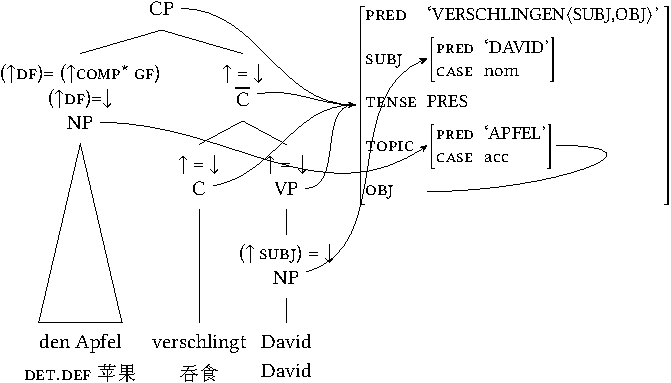
\includegraphics{Figures/den-apfel-verschlingt-david-lfg-lsp-crop}
}
\caption{\label{Abbildung-V2-LFG}动词二位的分析}
%\caption{\label{Abbildung-V2-LFG}Analysis of verb second}
\end{figure}%
\end{enumerate}

%\pagebreak
\section{范畴语法}
%\section{Categorial Grammar}

%\largerpage
\begin{enumerate}
\item The children in the room laugh loudly.的分析如图~\ref{Abbildung-CG-Kinder-lachen-laut}所示。
%\item The analysis of \emph{The children in the room laugh loudly.} is given in Figure~\ref{Abbildung-CG-Kinder-lachen-laut}.
\begin{figure}[H]
\centerline{%
\deriv{7}{
the   & children  & in  & the      & room                 & laugh & loudly\\
\textsc{art}.\textsc{def}   & \textrm{孩子们}  & \textsc{prep}  & \textsc{art}.\textsc{def}    & \textrm{房间}   & \textrm{笑} & \textrm{大声}\\
\hr   & \hr       & \hr & \hr      & \hr                    & \hr     & \hr \\
%
%
np/n  & n       & (n\bs n)/np & np/n & n                & s\bs np  & (s\bs np)\bs (s\bs np)\\
      &         &             & \multicolumn{2}{c}{\forwardapp} & \multicolumn{2}{c@{}}{\backwardapp}\\
      &         &             & np\\
      &         & \multicolumn{3}{c}{\forwardapp}  & \multicolumn{2}{c@{}}{s\bs np}\\
%
%
      &         & \multicolumn{3}{c}{n\bs n} \\  
      & \multicolumn{4}{c}{\backwardapp}\\
      & \multicolumn{4}{c}{{{n}}}\\
%
\multicolumn{5}{@{}c}{\forwardapp}\\
\multicolumn{5}{@{}c}{{np}}\\
%
\multicolumn{7}{@{}c@{}}{\backwardapp}\\
\multicolumn{7}{@{}c@{}}{{s}}\\
}}
\caption{\label{Abbildung-CG-Kinder-lachen-laut}The children in
    the room laugh loudly.的范畴语法分析}
%\caption{\label{Abbildung-CG-Kinder-lachen-laut}Categorial Grammar analysis of \emph{The children in
%    the room laugh loudly.}}
\end{figure}%

\item the picture of Mary的分析如图\vref{Abbildung-CG-das-Bild-von-Maria}所示。n/pp对应于\nnull,n对应于\nbar ,而np对应于NP。
%\item The analysis of \emph{the picture of Mary} is given in
%  Figure~\vref{Abbildung-CG-das-Bild-von-Maria}. n/pp corresponds to \nnull, n corresponds to \nbar
%  and np corresponds to NP.
\begin{figure}[H]
\centerline{%
\deriv{4}{
the & picture & of & Mary\\
\textsc{art}.\textsc{def} & \textrm{照片}  & \textsc{prep} & Mary\\
\hr   & \hr     & \hr        & \hr\\
np/n  & n/pp    & pp/np      & np\\
%
      &         & \multicolumn{2}{c@{}}{\forwardapp}\\
      &         & \multicolumn{2}{c@{}}{pp}\\
%
      & \multicolumn{3}{c@{}}{\forwardapp}\\
      & \multicolumn{3}{c@{}}{n}\\
%
\multicolumn{4}{@{}c@{}}{\forwardapp}\\
\multicolumn{4}{@{}c@{}}{np}\\
}}
\caption{the picture of Mary\label{Abbildung-CG-das-Bild-von-Maria}的范畴语法分析}
%\caption{Categorial Grammar analysis of \emph{the picture of Mary}\label{Abbildung-CG-das-Bild-von-Maria}}
\end{figure}%
\end{enumerate}

%\pagebreak

\section{中心语驱动的短语结构语法}
%\section{Head-Driven Phrase Structure Grammar}

%\largerpage
\begin{enumerate}
\item 答案是:\\[1mm]
%\item The solution is:\\[1mm]
%\vpageref{avm-max-lacht}.
%\begin{figure}
\oneline{%
\onems[head-argument-phrase~]{
      phon  \phonliste{ Max lacht }\\
      synsem$|$loc \ms{ cat \ms{ head & \ibox{1}\\
                                 subcat & \ibox{2} \eliste \\
                               }\\
                        cont \ms{ ind & \ibox{3}  \\
                                       rels & \relliste{ \ibox{4}, \ibox{5} } \\
                                     }\\
                      }\\
      head-dtr \onems[word]{ phon \phonliste{ lacht }\\
                             synsem$|$loc  \ms{ cat & \ms{ head   & \ibox{1} \ms[verb]{ initial & $-$\\
                                                                                        vform   & fin \\
                                                                                   }\\
                                                            subcat & \ibox{2}  $\oplus$ \sliste{ \ibox{6} }  \\
                                                        }\\
                                                 cont & \ms{ ind & \ibox{3} event \\
                                                                  rels & \liste{ \ibox{4} \ms[lachen]{ event & \ibox{3} \\
                                                                                                       agens & \ibox{7} \\ }} \\
                                                                }
                                               }\\
                       } \\
      non-head-dtrs \liste{ \onems[word]{ 
                                        phon \phonliste{ Max }\\
                                        synsem \ibox{6} \onems{ loc \ms{ cat & \ms{ head   & \ms[noun]{ cas & nom\\
                                                                                                      } \\
                                                                                    subcat &  \eliste \\
                                                                                }\\
                                                                         cont & \ms{ ind & \ibox{7} \ms{ per & 3 \\
                                                                                                              num & sg \\
                                                                                                              gen & mas \\
                                                                                                            } \\
                                                                                          rels & \liste{
                                                                                                  \ibox{5} \ms[named]{ name & max    \\
                                                                                                                       inst & \ibox{7} \\ }} \\
                                                                                         } \\
                                                                        }\\
                                                              }\\
                                   } 
                           } \\
}}
\label{avm-max-lacht}
%\end{figure}%
\item 对于例(\mex{1})中的最小差比对儿的分析需要捕捉到这样的事实,形容词的格需要与名词的格保持一致。在(\mex{1}a)中,我们使用了interessant(有趣的)的属格形式,而(\mex{1}b)包含的形式是与属格的单数不相容的形式。
%\item An analysis of the difference in (\mex{1}) has to capture the fact that the case of the adjective has to %agree with that of the noun. In (\mex{1}a),
%the genitive form of \emph{interessant} `interesting' is used, whereas (\mex{1}b) contains a form that is %incompatible with the genitive singular.
\eal
\ex[]{
\gll eines interessanten Mannes\\ 
     一.\gen{} 有趣的.\gen{} 男人.\gen{}\\
%     one.\gen{} interesting.\gen{} man.\gen{}\\
}
\ex[*]{ 
\gll eines interessanter Mannes\\
     一.\gen{} 有趣的.\nom{} 男人.\gen{}\\
%     one.\gen{} interesting.\nom{} man.\gen{}\\
}
\zl
\par\setlength\parindent{2em}
(\mex{1})说明了interessanten的\catvc 。 
%(\mex{1}) shows the \catv of \emph{interessanten}.

\eas
带有格信息的interessanten(有趣的)的\catvc  :\\
%\catv of \emph{interessanten} `interesting' with case information:\\
\ms{ head & \ms[adj]{ %prd & $-$ \\
                      mod  & {\upshape \nbar[\textsc{case} \ibox{1}]}\\
                      case & \ibox{1} gen\\
                    } \\
              subcat & \liste{} \\
}
\zs
在\textsc{mod}下形容词的格的取值与\nbar 的格的取值的结构共享决定了名词和形容词的格的取值。由此,interessanten可以跟Mannes组合,但是不能跟Mann组合。类似地,interessanter只能跟主格的Mann组合,而不能跟属格的Mannes组合。
%The structure sharing of the case value of the adjective with the case value of the \nbar under \textsc{mod}
%identifies the case values of the noun and the adjective. \emph{interessanten} can therefore be combined with 
%\emph{Mannes}, but not with \emph{Mann}. Similarly, \emph{interessanter}
%can only be combined with the nominative \emph{Mann}, but not with the genitive \emph{Mannes}. 
\par\setlength\parindent{2em}
对于名词短语内部一致关系的改进,参见 \citew[\S~13.2]{MuellerLehrbuch1}。
%For a refinement of the analysis of agreement inside the noun phrase, see  \citew[Abschnitt~13.2]
%{MuellerLehrbuch1}.
\end{enumerate}


\section{构式语法}
%\section{Construction Grammar}

熟语可以通过仔细阅读报纸来获得。稍微枯燥的方法是查找熟语词典,如“熟语与短语免费辞典”\footnote{%
\url{http://idioms.thefreedictionary.com/},\zhdate{2015/03/04}。
}。
%Idioms can be found by reading the newspaper carefully. The less exciting method is to look them up a %dictionary of
%idioms such as the Free Dictionary of Idioms and Phrases\footnote{%
%\url{http://idioms.thefreedictionary.com/}, 04.03.2015.
%}.


\section{依存语法}
%\section{Dependency Grammar}

\begin{figure}[H]
\centering
\scalebox{.9}{%
\begin{forest}
dg edges
[V
  [N [ich;我]]
  [habe;\textsc{aux}]
  [N,name=n
    [Det,tier=det [einen;一个]]
    [Mann;男人]]
  [V [getroffen;遇见]]
  [Rel,no edge, tier=det,name=rel [\trace]
      [V
        [N [der;\textsc{rel}]]
        [N [Adj, dg adjunct [blonde;金色]]
           [Haare;头发]]
        [hat;有]]]]
\draw (n.south)--(rel.north)-- +(0,6pt);
\end{forest}
}
\end{figure}%

\begin{figure}[H]
\centering
\scalebox{.9}{%
\begin{forest}
dg edges
[V
  [Subjunction
    [dass;\textsc{comp}]
    [V, l sep+=15pt
      [N [er;他]]
      [Adv, dg adjunct [morgen;明天]]
      [V [kommen;来]]
      [wird;将]]]
  [freut;高兴]
  [N [uns;我们]]]
\end{forest}
}
\end{figure}%

\begin{figure}[H]
\centering
\scalebox{.9}{
\begin{forest}
dg edges
[V
  [V [N,name=n
       [Det,tier=det [einen;一个]]
       [Mann;男人]]
    [getroffen;遇见]]
  [Rel,no edge, tier=det,name=rel [\trace]
      [V
        [N [der;\textsc{rel}]]
        [N [Adj, dg adjunct [blonde;金色]]
           [Haare;头发]]
        [hat;有]]]
  [habe;\textsc{aux}]
  [N [ich;我]]
  [Adv [noch;还]]
  [Adv [nie;从不]]]
\draw (n.south)--(rel.north)-- +(0,6pt);
\end{forest}
}
\end{figure}%






\section{树邻接语法}
%\section{Tree Adjoining Grammar}

(\mex{1})的分析需要图\vref{TAG-Elementarbaeume-dem-Koenig-treue}中的基本树。
%The elementary trees in Figure~\vref{TAG-Elementarbaeume-dem-Koenig-treue} are needed for the analysis of (\mex{1}).
\ea
\gll der        dem        König treue Diener\\
     \textsc{art}.\textsc{def}.\nom{} \textsc{art}.\textsc{def}.\dat{} 国王  忠诚 仆人\\
\mytrans{对国王忠诚的仆人}
%     the.\nom{} the.\dat{} king  loyal servant\\
%\mytrans{the servant loyal to the king}
\z

\begin{figure}
\hfill
\scalebox{.9}{
\begin{forest}
tag
[Det [der;\textsc{art}.\textsc{def}]]
\end{forest}
}
\hfill
\scalebox{.9}{
\begin{forest}
tag
[Det [dem;\textsc{art}.\textsc{def}]]
\end{forest}
}
\hfill
\scalebox{.9}{
\begin{forest}
tag
[NP
  [Det$\downarrow$]
  [N$'$
    [N [König;国王]]]]
\end{forest}
}
%
\hfill
%
\scalebox{.9}{
\begin{forest}
tag
[N$'$
  [AP
    [A$'$
      [NP$\downarrow$]
      [A [treue;忠诚]]]]
  [N$'$*]]
\end{forest}
}
%
\hfill
%
\scalebox{.9}{
\begin{forest}
tag
[NP
  [Det$\downarrow$]
  [N$'$
    [N [Diener;仆人]]]]
\end{forest}
}
\hfill\mbox{}
\caption{\label{TAG-Elementarbaeume-dem-Koenig-treue}der dem König treue Diener的基本树}
%\caption{\label{TAG-Elementarbaeume-dem-Koenig-treue}Elementary trees for \emph{der dem König treue Diener}}
\end{figure}%

%\noindent
\par\setlength\parindent{2em}
通过在替换结点König(国王)替换dem的树,我们会得到一个完整的NP。然后,这就可以插进treue(忠诚的)的替换结点中。相似地, der的树可以跟Diener的树组合。然后,我们就得到图\vref{TAG-substituiert}中的两棵树了。
%By substituting the tree for \emph{dem} `the' in the substitution node of \emph{König} `king', one then arrives at a full NP.
%This can then be inserted into the substitution node of \emph{treue} `loyal'. Similarly, the tree
%for \emph{der} `the' can be combined with the one for \emph{Diener}. One then has both of the trees in Figure~\vref{TAG-substituiert}.

\begin{figure}
\hfill
\scalebox{.9}{
\begin{forest}
tag
[N$'$
  [AP
    [A$'$
      [NP
        [Det [dem;\textsc{art}.\textsc{def}]]
        [N$'$
          [N [König;国王]]]]
      [A [treue;忠诚]]]]
  [N$'$*]]
\end{forest}
}
%
\hfill
\scalebox{.9}{
\begin{forest}
tag
  [NP
     [Det [der;\textsc{art}.\textsc{def}]]
     [N$'$
        [N [Diener;仆人]]]]
\end{forest}
}
\hfill\mbox{}
\caption{\label{TAG-substituiert}替换后的der dem König treue树和der Diener树}
%\caption{\label{TAG-substituiert}Trees for \emph{der dem König treue} and \emph{der Diener} after substitution}
\end{figure}%
\par\setlength\parindent{2em}
形容词树可以连接到der Diener的N$'$"=n结点上,并得到图\vref{TAG-Baeume-nach-Adjunktion}中的结构。
%The adjective tree can then be adjoined to the N$'$"=node of \emph{der Diener}, which yields the structure in Figure~\vref{TAG-Baeume-nach-Adjunktion}.
\begin{figure}
\centering
%\scalebox{.9}{
\begin{forest}
tag
  [NP
     [Det [der;\textsc{art}.\textsc{def}]]
     [N$'$
       [AP
         [A$'$
           [NP
             [Det [dem;\textsc{art}.\textsc{def}]]
             [N$'$
               [N [König;国王]]]]
           [A [treue;忠诚]]]]
       [N$'$
         [N [Diener;仆人]]]]]
\end{forest}
%}
\caption{\label{TAG-Baeume-nach-Adjunktion}将AP附加到N$'$"=结点的结果}
%\caption{\label{TAG-Baeume-nach-Adjunktion}Result of adjunction of the AP to the N$'$"=node}
\end{figure}%




%      <!-- Local IspellDict: en_US-w_accents -->
